\chapter{Algorithms and Approaches for Terrain LOD}
\section{ROAM}
\textit{ROAM} (short for \textbf{R}eal-time \textbf{O}ptimally \textbf{A}dapting \textbf{M}eshes) 
is a terrain LOD algorithm developed by Duchaineau \textit{et al.} \cite{roam} published in 1997.
ROAM represents the terrain mesh using bintrees and performs triangle splits and merges
for generating and removing detail. 
The splits and merges happen mainly on the CPU, which makes ROAM a mainly CPU-based approach.

\subsection{General Idea}
The central idea of the algorithm is to use temporal coherence: the mesh from a previous frame $\mathbf{T}_{f-1}$ is used to compute 
the mesh of the current frame $\mathbf{T}$, rather than building up the mesh from ground up for each frame.
This is done using two priority queues: a split queue $\mathcal{Q}_s$ and a merge queue $\mathcal{Q}_m$.
The split queue contains splittable triangles $T$
and the merge queue contains mergable triangle pairs $(T,T_B)$.
The elements of the priority queues are ordered by 
various geometric error metrics, which are explained in the subsection ``Error Metrics'' of this report.
At each frame, the terrain mesh gets split and merged using $\mathcal{Q}_s$ and $\mathcal{Q}_m$. until either the required size/accuracy is reached
or the time runs out.
ROAM is designed as a greedy algorithm, meaning it will always performs the most optimal splits/merges for each frame.

\subsection{Error Metrics}
The original ROAM paper mentions various error metrics for the priority queue ordering,
which are explained in the following paragraphs.

\paragraph{Wedgies} \textit{Wedgies} are nested bounding volumes around triangles that are computed 
while building the initial mesh at the beginning of the algorithm.
A wedgie is defined to contain the entire $x$ and $z$ extent\footnote{The original ROAM paper uses $z$ for the up direction. For the sake of consistency with the rest of this report, we will use $y$ as the up direction here.}
of a triangle and the height $y$ including some additional space above and below the highest and lowest points,
respectively.

\paragraph{Geometric Screen Distortion}
Another metric is the distance between where a node is supposed to be on the screen and where the algorithm placed the node.
The maximum of all distances is calculated and used as the base priority metric of the algorithm.

\subsection{Other Optimizations}
\paragraph{View-frustum Culling}
An optimization that is mentioned is view-frustum culling. In each frame, various flags are updated during 
the recursive traversal of the bintree. These flags indicate whether a wedgie is inside the view-frustum 
fully, partially, or not at all.

\paragraph{Incremental Triangle Stripping}
The ROAM paper reports using \textit{incremental triangle stripping} for optimizing the performance of the rendering.
This is simply refers to using triangle strips for rendering. which is supported by all major graphics APIs.

\subsection{Conclusion}
The runtime of ROAM is independent of the screen resolution and is proportional to the 
number of triangle changes per frame. 

%\section{Röttger's Quadtree-based Algorithm}
%TODO

\section{GeoMipMapping}
\textit{Geometrical Mipmapping (GeoMipMapping)} is a terrain LOD approach developed by de Boer \cite{geomipmapping} in the year 2000. 
It applies the idea of texture mipmapping to terrain rendering. In this section, all 
presented ideas are from the original paper, unless noted otherwise.

\subsection{General Idea}
The central idea of GeoMipMapping is its analogy to texture mipmapping: just like how textures of far away objects are rendered using lower resolution texture mipmaps,
terrain areas that are far away from the camera should also be rendered with a lower resolution mesh.

This is achieved by splitting up the terrain into so-called \textit{blocks} (also called \textit{patches}) of a fixed width $2^n + 1$ for an arbitrary $n \in \mathbb{N}$.
Each block has a LOD level\footnote{The original GeoMipMapping paper uses 0 to denote the maximum LOD level and vice-versa for the minimum LOD level. In order to avoid any confusion with the term \textit{LOD}, this report denotes 0 as the minimum LOD level and vice versa for the maximum LOD level.} $0\leq l \leq n$ that changes dynamically at runtime.
At load time, every block is computed at every LOD level and subsequently stored, e.g. on an index buffer.
Each such representation of a block at a specific LOD level is called a \textit{GeoMipMap}.
For each GeoMipMap, the number of vertices on one side is $2^{l}+1$ and the number of quads is $2^{2l}$.

For example, the GeoMipMaps of a $5 \times 5$ terrain block contain $2^2 + 1 = 5$ vertices on one side at the maximum LOD level 2, $2^1 + 1 = 3$ vertices at LOD level 1 and $2^0 + 1 = 2$ vertices at the minimum LOD level 0.
As for the number of quads, at LOD level 2 there are $2^{4} = 16$ quads, at LOD level 1 there are $2^2 = 4$ quads and at LOD level 0 there is $2^0 = 1$ quad.
Figure~\ref{fig:geomipmapping-patch-example} illustrates the above example.

% \begin{figure}[H]
%   \centering
%   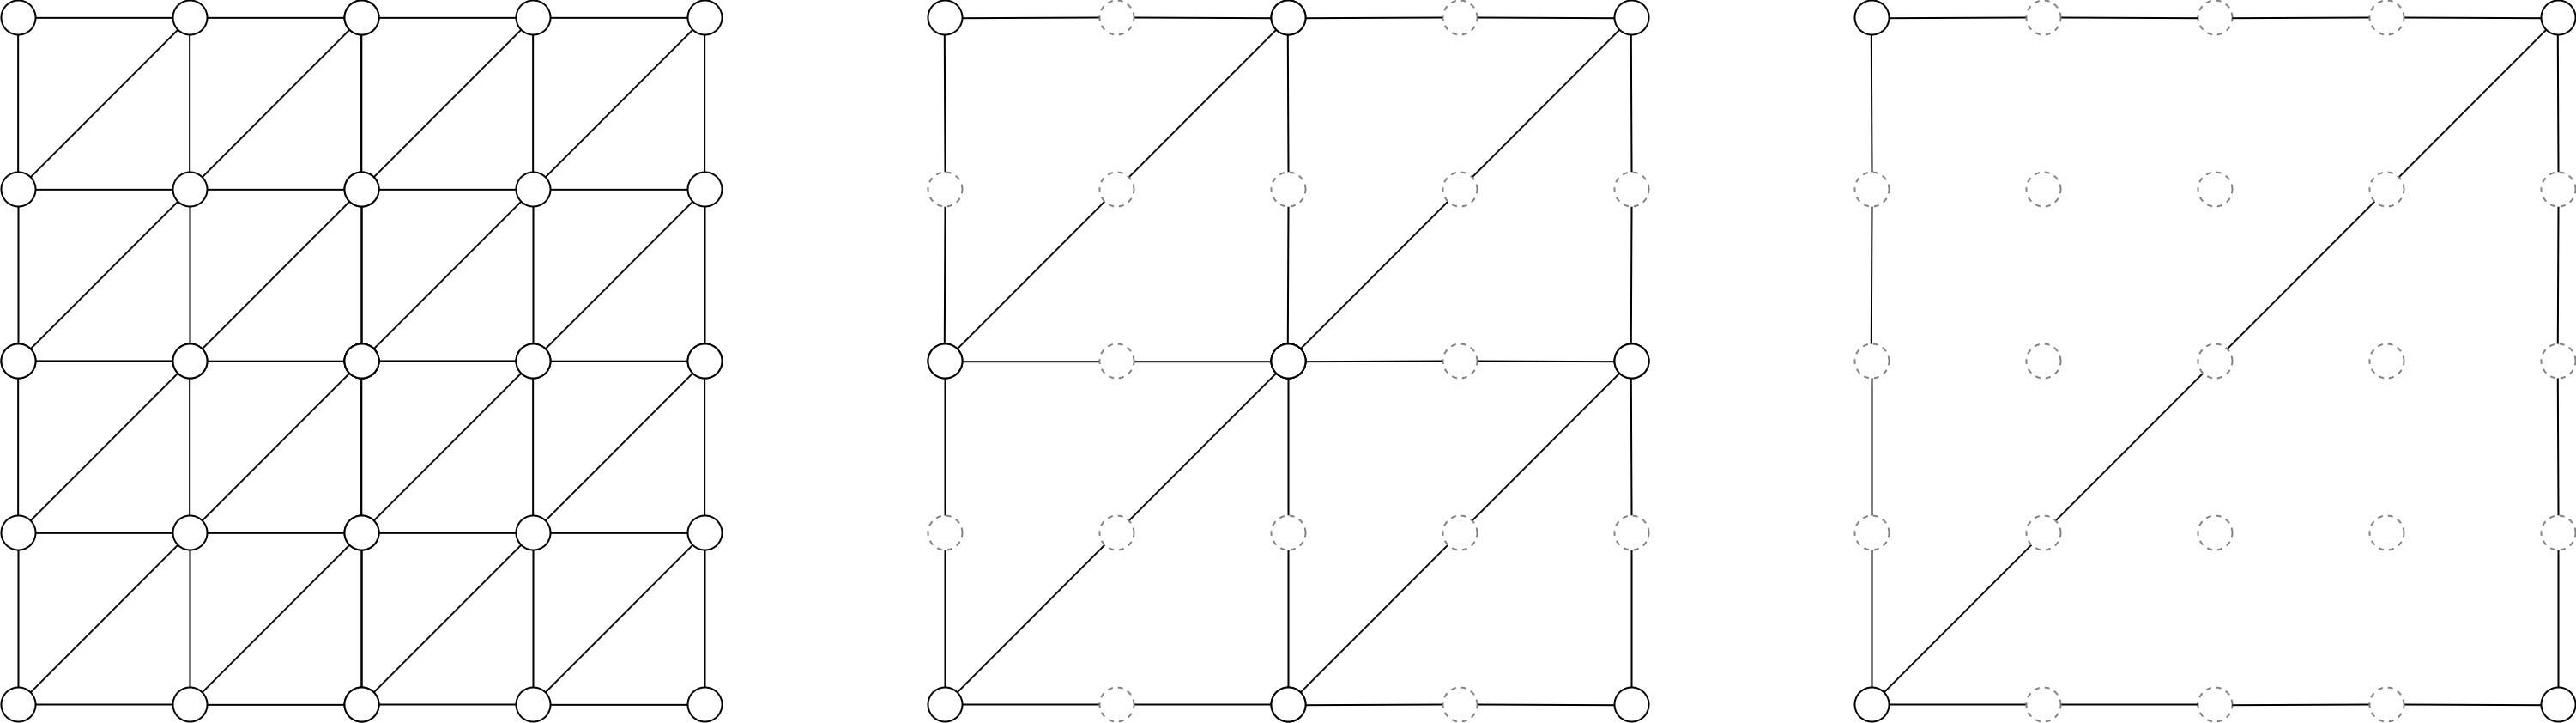
\includegraphics[width=1\textwidth]{geomipmapping-patch-example}
%   \caption{Example of a $5 \times 5$ block at the maximum LOD level of 2 (left), LOD level of 1 (middle) and minimum LOD level of 0 (right). The omitted vertices of the lower LOD blocks are shown here as dotted circles.}\label{fig:geomipmapping-patch-example}
% \end{figure}

\begin{figure}[H]
  \centering
  \subfloat[\centering LOD level 2 (maximum).]{{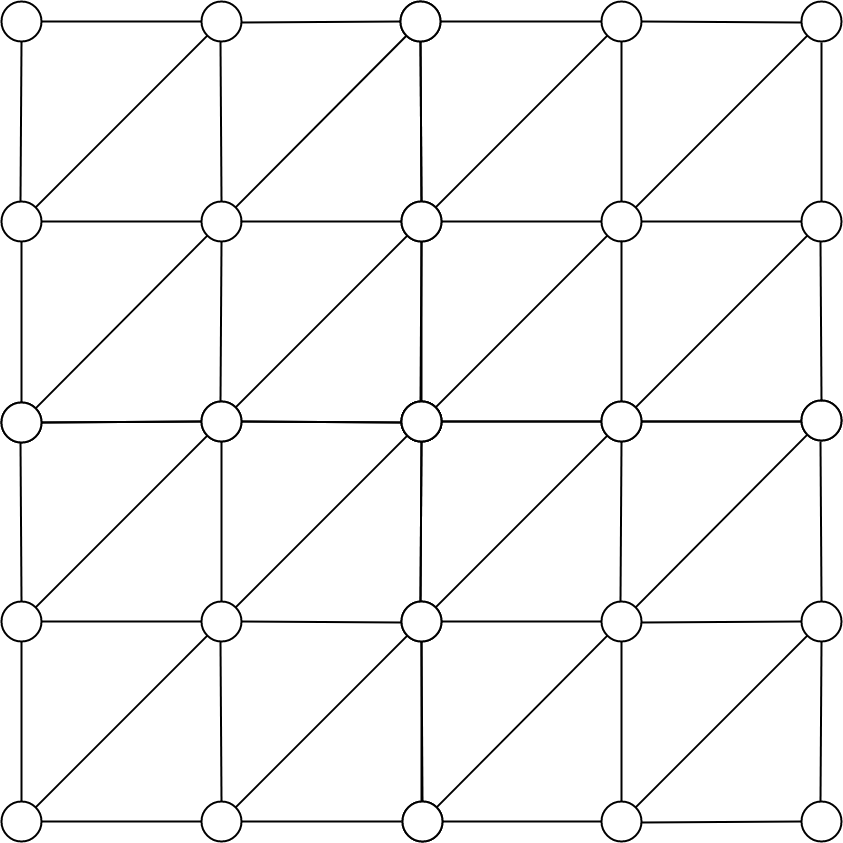
\includegraphics[width=0.28\textwidth]{geomipmapping-level-2.png} }}
  \qquad
  \subfloat[\centering LOD level 1.]{{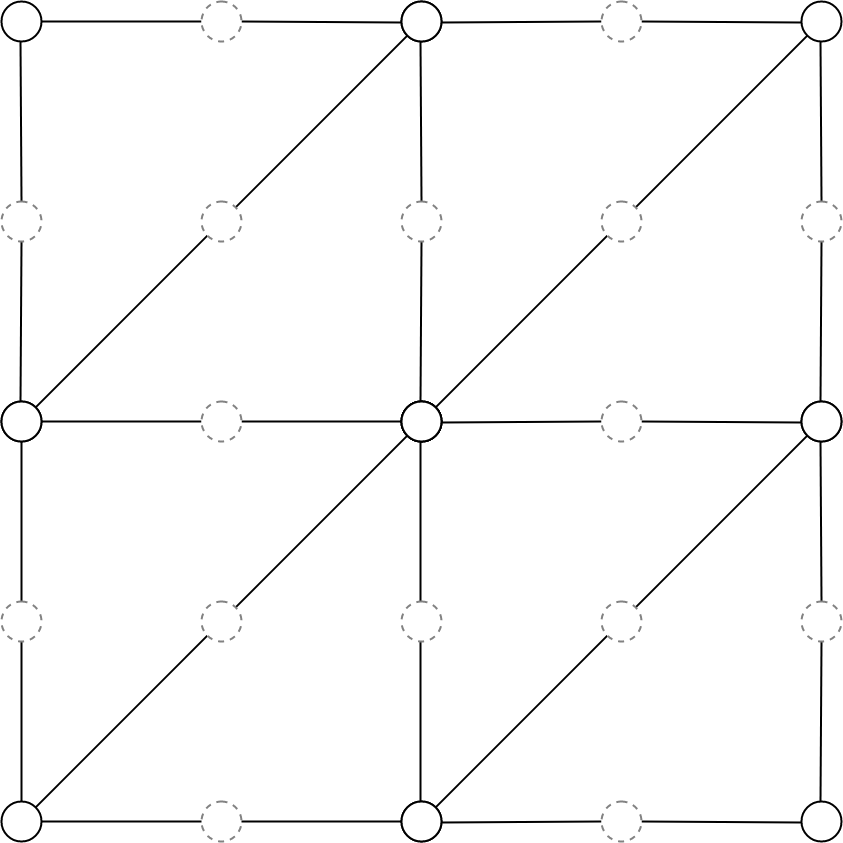
\includegraphics[width=0.28\textwidth]{geomipmapping-level-1.png} }}
  \qquad
  \subfloat[\centering LOD level 0 (minimum).]{{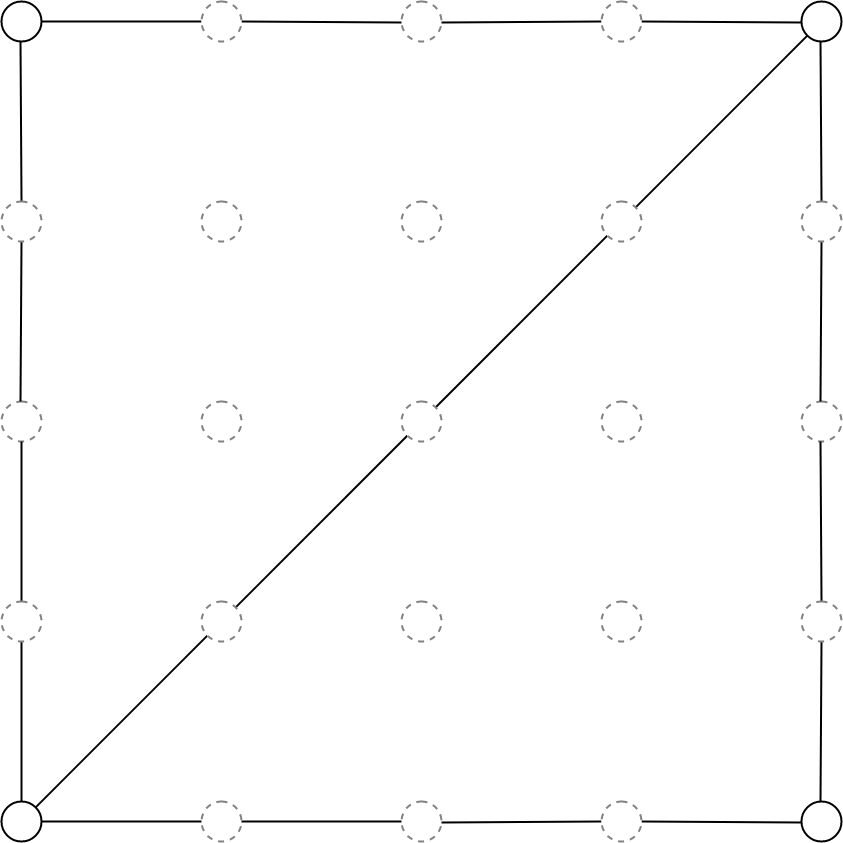
\includegraphics[width=0.28\textwidth]{geomipmapping-level-0.png} }}
  \caption{Example of each GeoMipMap of a $5 \times 5$ block. The omitted vertices of lower LOD GeoMipMaps are marked as dotted circles.}\label{fig:geomipmapping-patch-example}
\end{figure}

\subsection{View-frustum Culling}
The organisation of the terrain into blocks allows for easy view-frustum culling,
which dramatically decreases the number of vertices that need to get rendered.


\subsection{LOD Selection}
The LOD for each block is selected at runtime and is based on a 

\subsection{Avoiding Cracks}
GeoMipMapping avoids cracks by checking whether the
current block has a higher LOD than the bordering block and if this is the case,
it omits the vertices that would cause the crack.
The vertex omission is performed by rendering the bordering row/column of the current block
as triangle fans, as shown in figure~\ref{fig:geomipmapping-crack-avoidance}.

\begin{figure}[H]
  \centering
  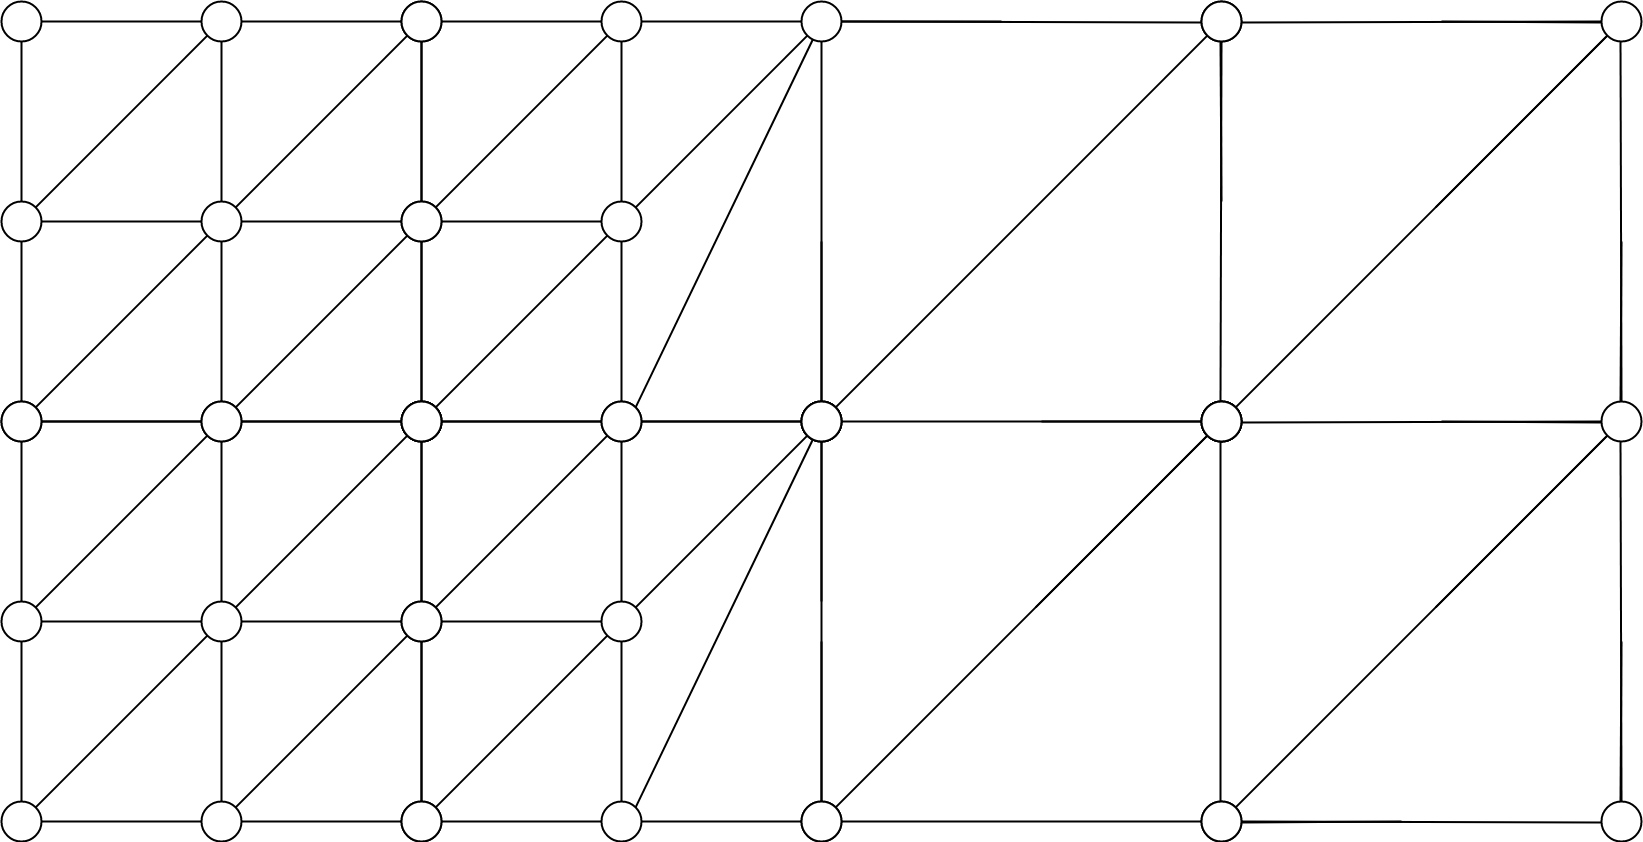
\includegraphics[width=0.7\textwidth]{geomipmapping-crack-avoidance}
  \caption{Example of GeoMipMapping's crack avoidance between a LOD 2 and a LOD 1 GeoMipMap of two $5 \times 5$ blocks as described in the original paper.}\label{fig:geomipmapping-crack-avoidance}
\end{figure}

% An alternative way to render neighboring blocks with different LOD levels is to render the triangle fans from the center point of each $3 \times 3$ border subblock. 
% This approach is somewhat simpler for handling special cases, e.g. when both the top and right neighboring blocks have a lower LOD,
% as shown shown in figure~\ref{fig:geomipmapping-crack-avoidance-alternative}.

%\begin{figure}[H]
%  \centering
%  \includegraphics[width=0.5\textwidth]{geomipmapping-crack-avoidance-alternative}
%  \caption{Alternative method to avoid cracks between a LOD 2 and a LOD 1 GeoMipMap of two $5 \times 5$ blocks.}\label{fig:geomipmapping-crack-avoidance-alternative}
%\end{figure}

\begin{figure}[H]
  \centering
  \subfloat[\centering Using the entire $3\times 3$ border subblocks for the triangle fans.]{{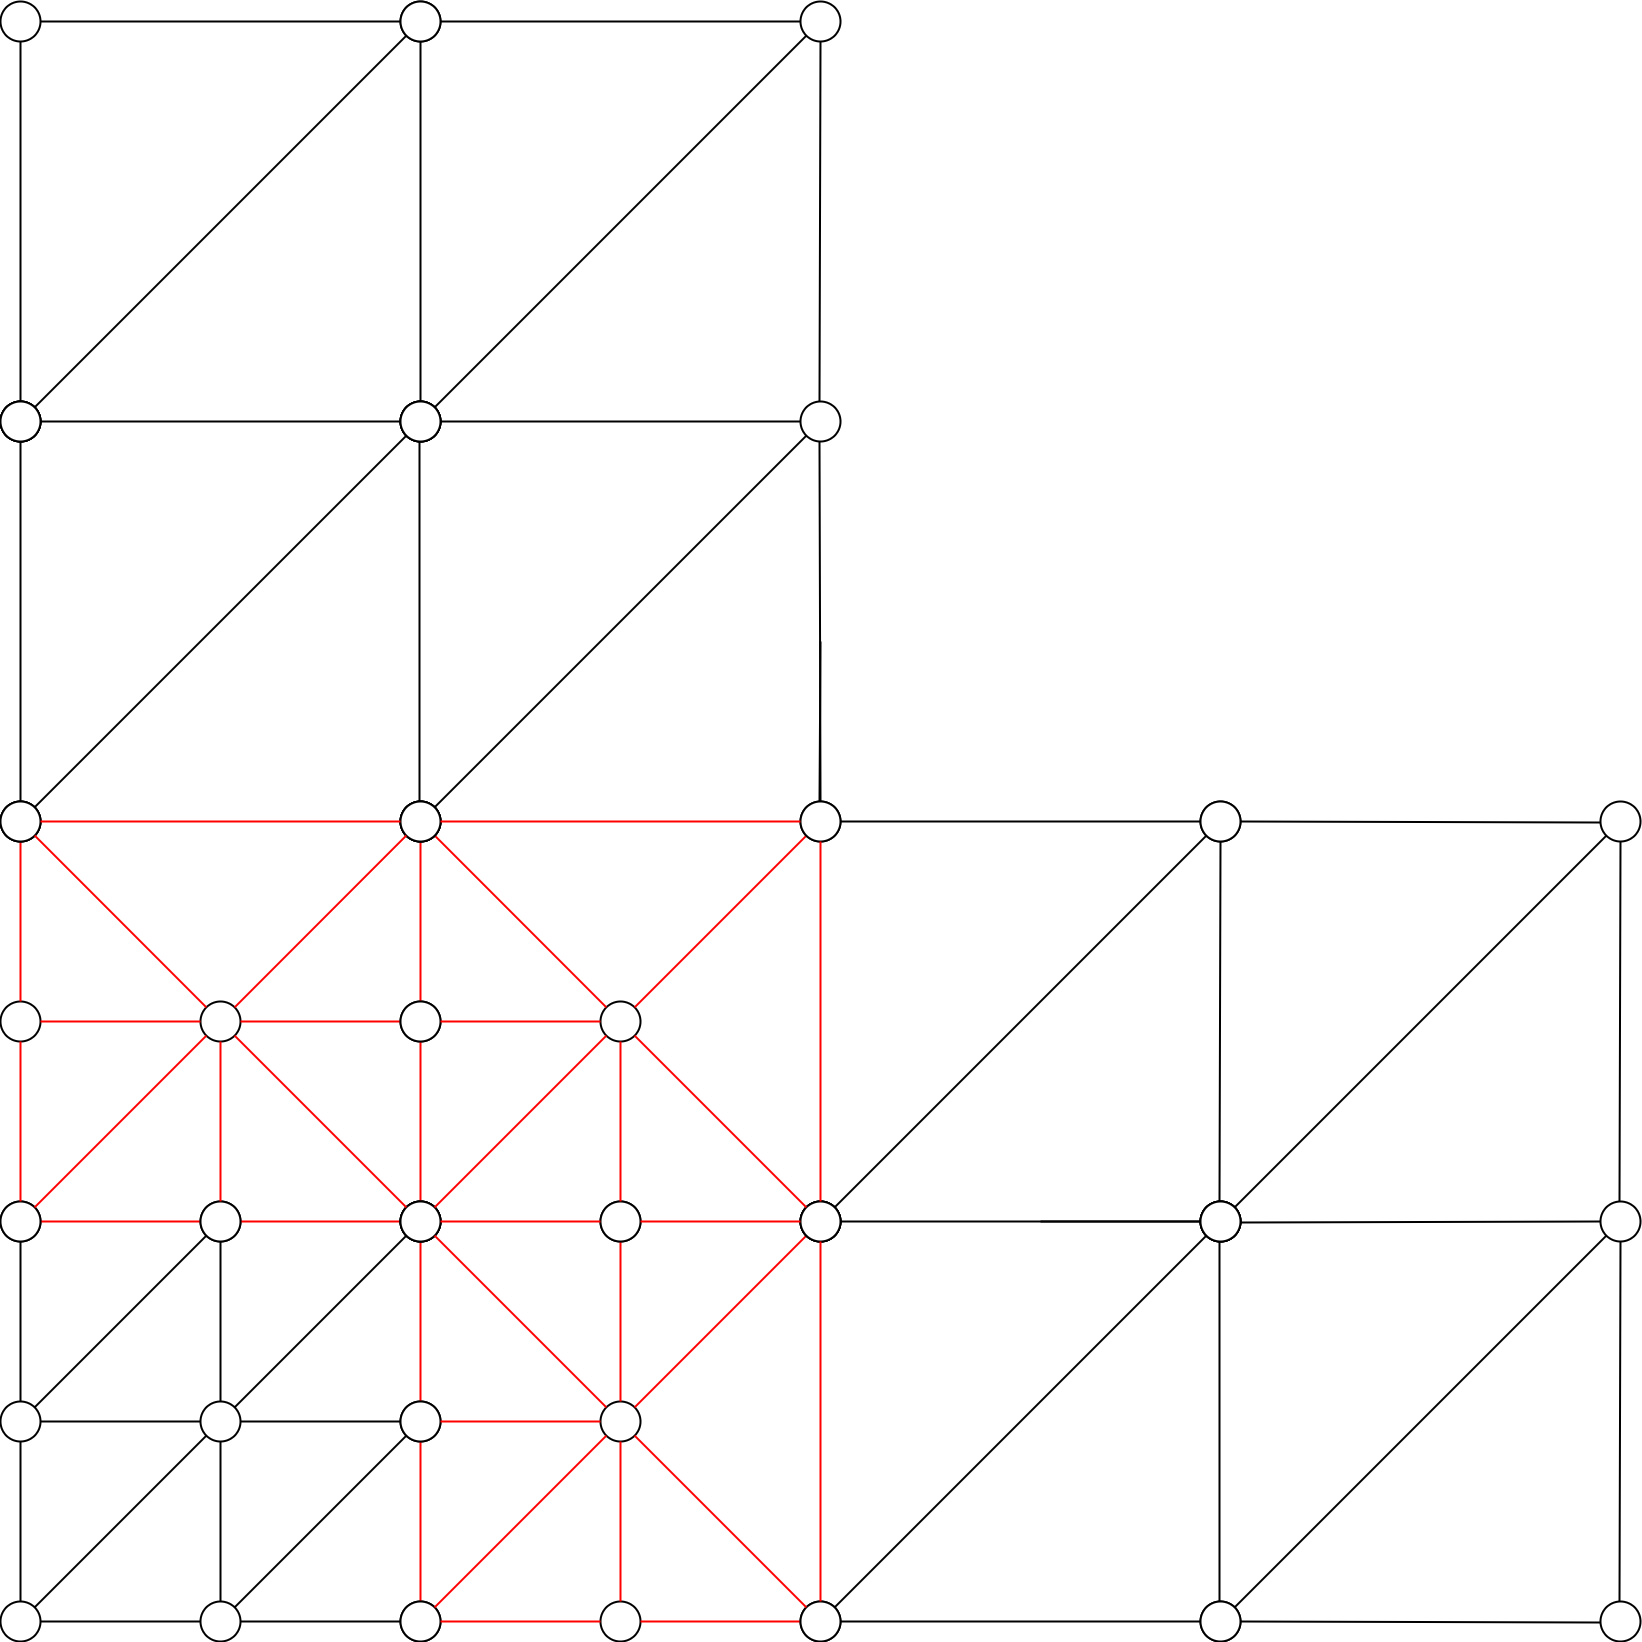
\includegraphics[width=0.45\textwidth]{geomipmapping-crack-avoidance-alternative-1} }}
  \qquad
  \subfloat[\centering Using only the top-most $2\times3$ subblocks and the right-most $3\times2$ subblocks for the triangle fans.]{{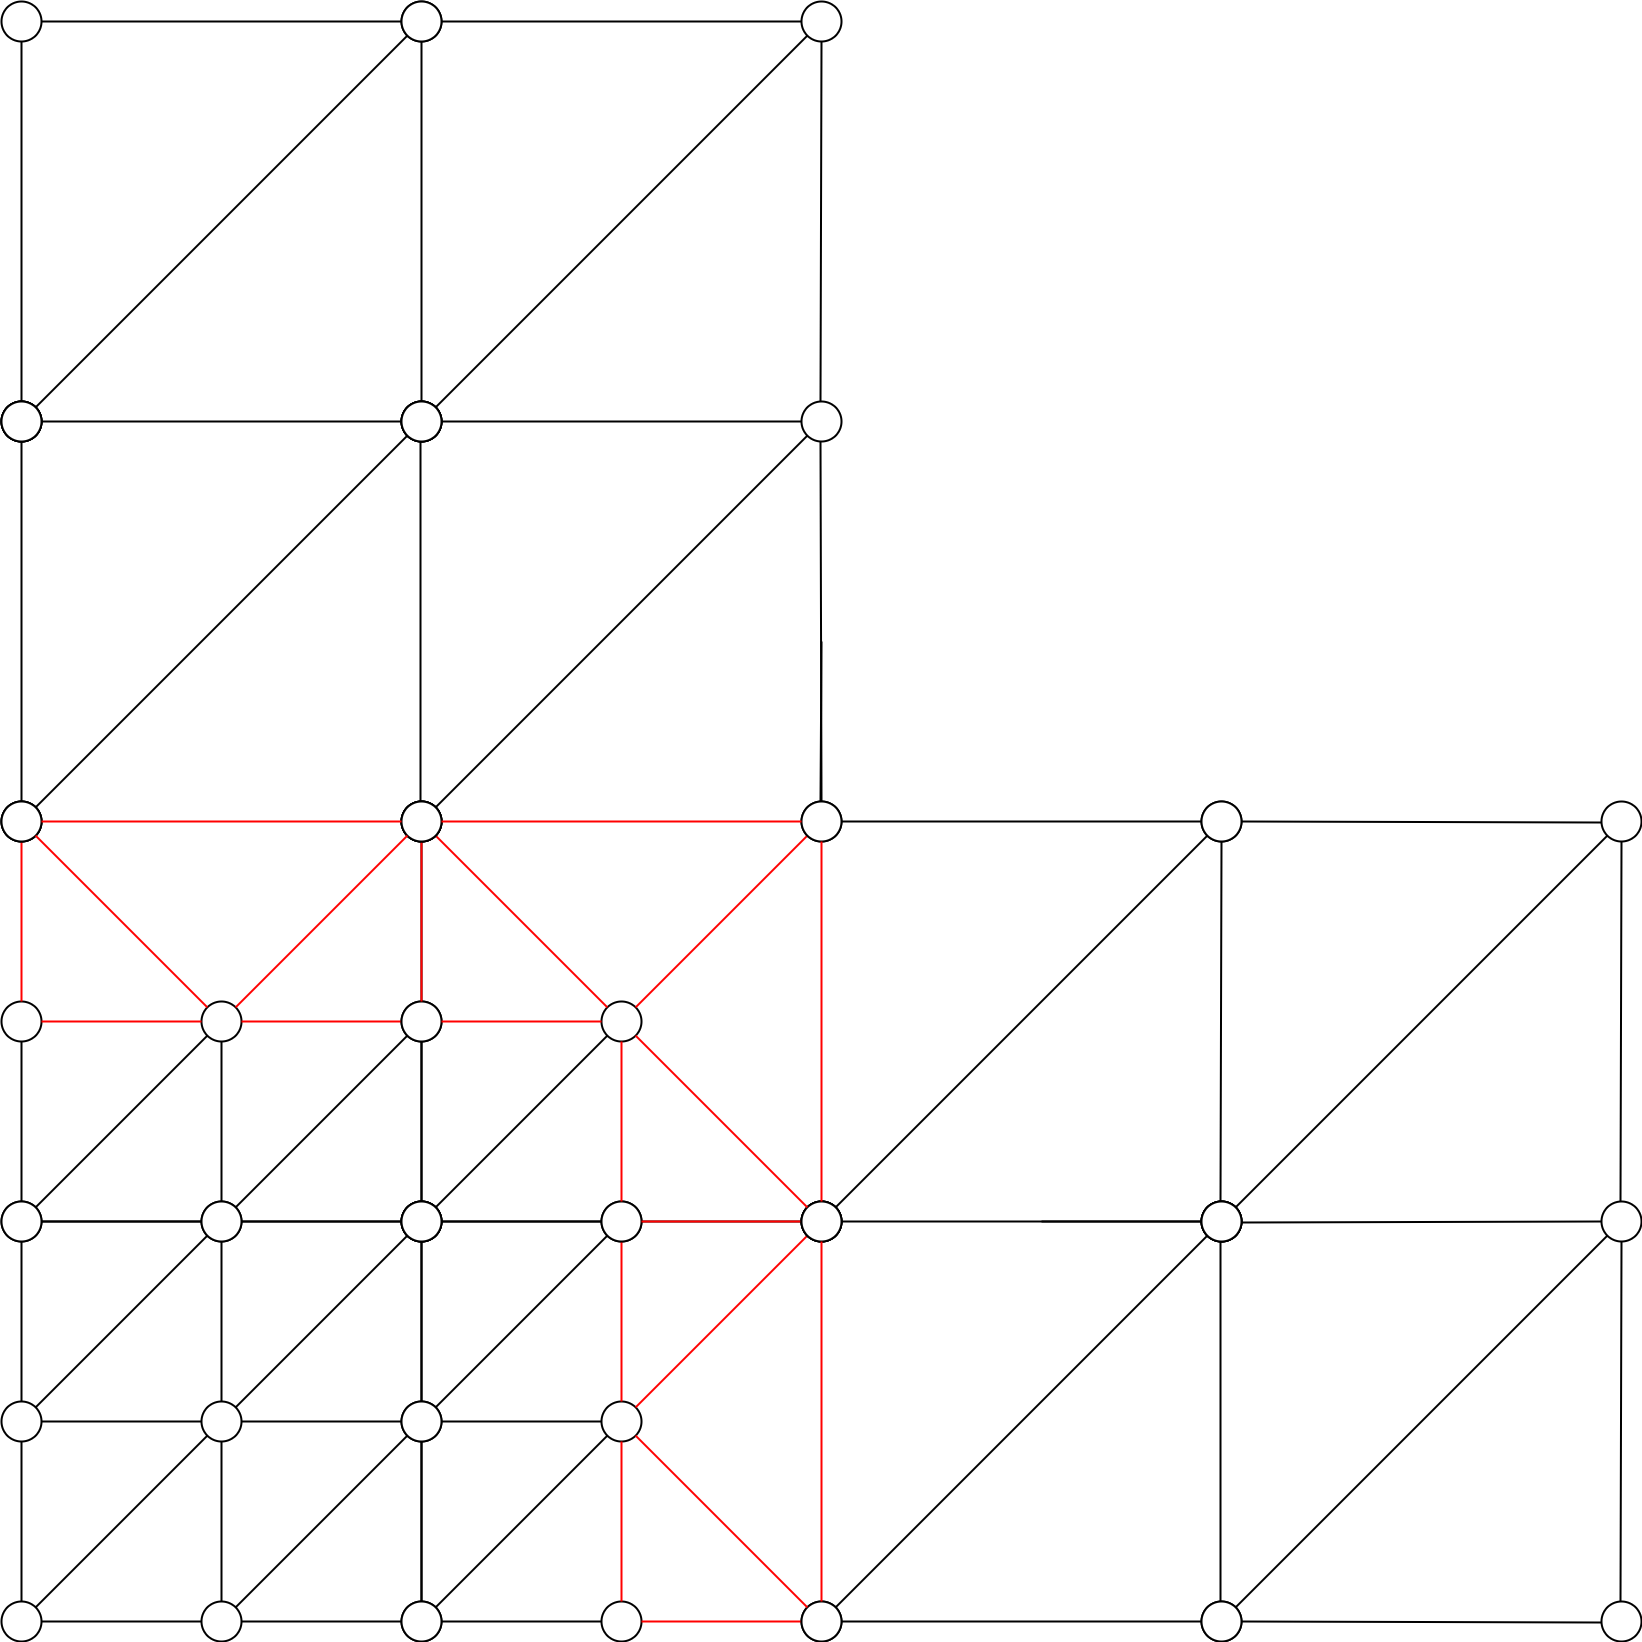
\includegraphics[width=0.45\textwidth]{geomipmapping-crack-avoidance-alternative-2} }}
  \caption{Two alternative triangle fan-based methods to avoid cracks between a LOD 2 and two LOD 1 GeoMipMaps of three $5 \times 5$ blocks. The border subblocks are marked in red.}\label{fig:geomipmapping-crack-avoidance-alternative}
\end{figure}

Regardless of the rendering approach, a neighborhood structure consisting of the LOD levels of the left, right, top and bottom 
neighboring blocks needs to be stored per block, so that the algorithm knows how to perform the vertex omission. The LOD levels of each block change continually each frame, which means 
that the neighborhood structure of each block also gets updated each frame.

\subsection{Other Optimizations}
\paragraph{Vertex Morphing}
GeoMipMapping can be extended with vertex morphing in order to decrease popping.




\section{Geometry Clipmaps}
Geometry Clipmaps is a terrain rendering technique published by Hoppe and Losasso in TODO.
The follow-up GPU-based 

%\section{CDLOD}
%TODO

\section{Concurrent Binary Trees}
TODO

\section{GPU Tessellation Shaders}

